\documentclass[border=10pt]{standalone}
\usepackage{tikz}
\begin{document}

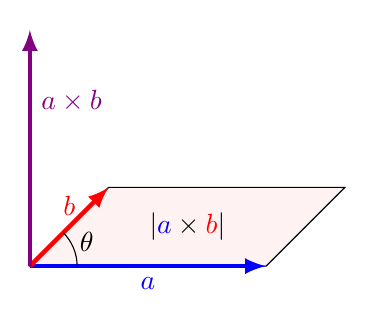
\begin{tikzpicture}
	\draw[-,fill=white!95!red](0,0)--(3,0)--(4,1)--(1,1)--cycle;
	\node at (2,0.5) {$|\textcolor{blue}{a}\times \textcolor{red}{b}|$};
	\draw[ultra thick,-latex,blue](0,0)--(3,0)node[midway,below]{$a$};
	\draw[ultra thick,-latex,red](0,0)--(1,1)node[midway,above]{$b$};
	\draw[ultra thick,-latex,blue!50!red](0,0)--(0,3)node[pos=0.7,right]{$a\times b$};
	\draw (0.6,0) arc [start angle=0,end angle=45,radius=0.6]
	node[pos=0.7,right]{$\theta$};
\end{tikzpicture}


\end{document}